\chapter{Outils d'analyse de défauts fonctionnels ESD}
\label{chap:4}

Jusqu'à présent, l'étude s'est focalisée sur le développement de méthodes pour l'acquisition de données de mesures.
Ce procédé est couteux et intervient tard dans le flot de conception.
Les outils de simulation en revanche sont utilisables dés le début du flot de conception.
Dans le contexte de la recherche de défaillance fonctionnelle, la simulation peut donc s'avérer très utile.
Néanmoins, les circuits intégrés dans le domaine automobile sont très complexes, avec de multiples niveaux de hiérarchie et une large quantité de fonctions analogiques.
Il n'est pas aisé de rechercher les points de défaillance de tels circuits intégrés.
C'est pourquoi des méthodes permettant de réduire la complexité du problème peuvent être d'une grande utilité dans cette recherche.
Dans ce chapitre, deux méthodes sont présentées.
La première méthode s'intéresse à la modélisation de blocs dans la puce exclusivement et à l'analyse de leurs interactions.
La seconde méthode cherche à développer un modèle boite-noire du circuit intégré en fonctionnement afin qu'il puisse être distribué aux équipementiers.
Le modèle leur permettrait de réaliser des simulations fonctionnelles ESD du circuit intégré sans nécessiter le design de la puce.

\section{Méthode hiérarchique intra-puce}

% What is bottom up
L'approche présentée ici est hiérarchique car elle s'intéresse à la modélisation de petits blocs de la puce, puis permet de connecter et combiner ces modèles pour prédire des défaillances à plus haut niveau.
Les modèles développés sont de type boite-noire, ils sont une représentation du comportement du bloc vu entre une entrée et une sortie, et font abstraction du design interne.
Cette approche présente l'intérêt que des fonctions individuelles sont susceptibles d'être réutilisées, et donc que l'effort de caractérisation et de modélisation n'a besoin d'être fourni qu'une seule fois.
Un schéma de caractérisation assez simple est utilisé en simulation pour caractériser chaque bloc (Fig. \ref{block_function_cz}).
Pour que des défaillances fonctionnelles puissent être détectées, le bloc doit être en fonctionnement.
Le setup d'injection prévoit également les connexions nécessaire pour l'alimenter, pour injecter sur une entrée un stress électrique et observer la réponse sur une sortie.
La charge de sortie $Z$ permet de tirer du courant sur la sortie si nécessaire.
La valeur de cette charge peut être définie à partir de la spécification du bloc.
Par exemple, si la sortie doit être connectée à des grilles de transistor, une très forte impédance est attendue et la charge $Z$ peut prendre une très valeur de l'ordre du G\textOmega{}.
L'impact de cette charge est étudié dans le document final et pour des fonctions analogiques il est généralement observé que l'impact est faible pendant la perturbation ESD.

\begin{figure}[!h]
  \centering
  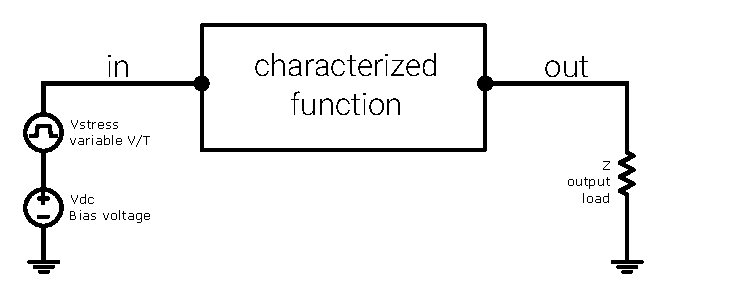
\includegraphics{src/1/figures/characterization_setup.pdf}
  \caption{Circuit de caractérisation de bloc}
  \label{block_function_cz}
\end{figure}

% What are the characterization signal
Le signal de caractérisation est une impulsion rectangulaire, appliquée sur l'entrée sous test.
Un ensemble de simulations est effectué en faisant varier les paramètres de cette forme d'onde, injectée sur l'entrée.
Plus précisément, une analyse paramétrique est réalisée sur l'amplitude et la durée de l'impulsion.
Cet ensemble de simulations est résumé dans la Fig. \ref{set_input_signals}.
Cette méthode de caractérisation est fortement inspirée de la méthode Wunsch & Bell \cite{wunsch-bell}.

\begin{figure}[!h]
  \centering
  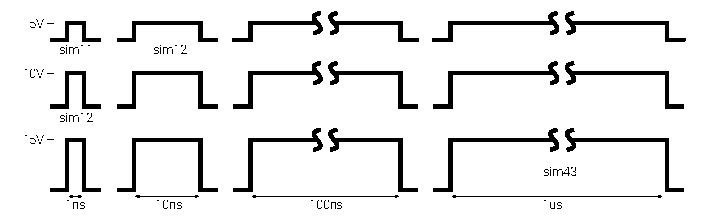
\includegraphics{src/1/figures/time_domain_cz_curves.pdf}
  \caption{Jeu de variations sur l'amplitude et la durée du signal de caractérisation}
  \label{set_input_signals}
\end{figure}

Deux paramètres sont extraits de la forme d'onde de sortie.
L'amplitude maximale et la durée de la perturbation observée sur la sortie sont enregistrées.
La durée correspond à 90\% de l'amplitude maximale relevée.
Ces deux paramètres permettent de décrire avec un signal rectangulaire plus simple que la forme d'onde de sortie.
Cette analyse est effectuée pour chaque simulation, et les résultats sont stockés dans deux tableaux.
Le premier tableau associe aux deux paramètres d'entrée (amplitude et durée) l'amplitude maximale de la perturbation sur la sortie.
Le second tableau associe aux deux paramètres d'entrée la durée de la perturbation sur la sortie.
Ces deux tables peuvent ensuite être intégrées dans un modèle, décrit Fig. \ref{fig:principle-transfert-func-v2}.
La fonction $F_{W}$ utilises la première table, pour retourner une amplitude de sortie en fonction des paramètres d'entrée.
La fonction $F_{V}$ utilises la seconde table et retourne une durée.
Sachant que ce modèle accepte les mêmes types de paramètres en entrée et en sortie, plusieurs modèles peuvent être chaînés les uns à la suite des autres.
En chainant les modèles de blocs, il est possible de reconstituer le comportement d'une fonction de plus haut-niveau composée de plusieurs blocs.

\begin{figure}[!h]
  \centering
  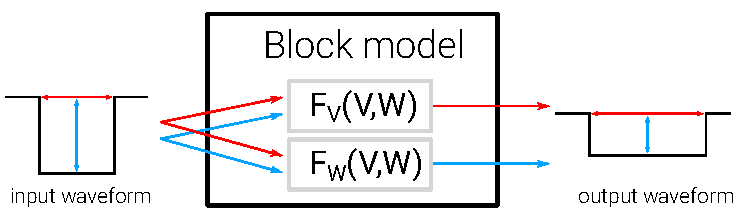
\includegraphics{src/1/figures/principle_transfert_function_v2.pdf}
  \caption{Méthode de modélisation améliorée}
  \label{fig:principle-transfert-func-v2}
\end{figure}

% First run the reference sim
Pour tester cette approche, des simulations sont effectuées en utilisant les schémas Fig. \ref{fig:hypothesis-setup}.
L'objectif est de comparer une simulation du schéma complet de la fonction, avec trois simulations individuelles.
Pour les simulations individuelles, l'amplitude et la durée de la perturbation d'une sortie sont utilisés comme stimulus pour la fonction suivante.
Par exemple, si une perturbation de -10V et 500ns est relevée sur la sortie du pré-régulateur, alors un stress de -10V 500ns est appliqué sur l'entrée du bloc suivant.

\begin{figure}[!h]
  \centering
  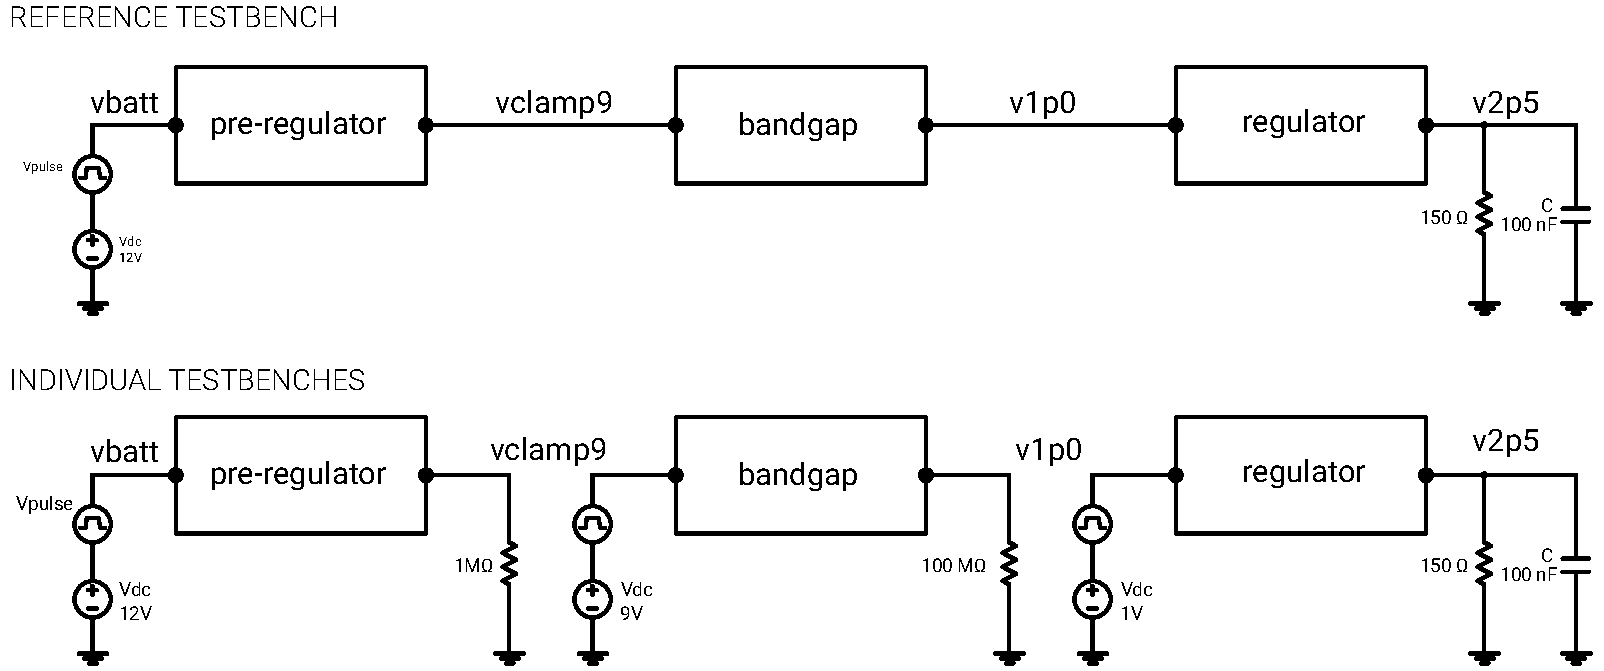
\includegraphics[width=0.98\textwidth]{src/1/figures/hypothesis_testing_setup.pdf}
  \caption{Schématique de validation de l'hypothèse}
  \label{fig:hypothesis-setup}
\end{figure}

% Then do the same thing but with the individual models
La courbe de la sortie du pré-régulateur simulé de manière individuelle (\textit{block 1 output}) est donnée Fig. \ref{fig:sim-compare-block1} et comparée avec la simulation totale (\textit{reference}).
Ces deux courbes corrèlent bien, malgré le fait qu'elle n'ont pas les mêmes charges en sortie.
Le stimulus appliqué sur le bandgap porte le label \textit{block 2 input} et représente le modèle simplifié de la courbe de sortie du pré-régulateur.
Le stimulus a pour amplitude maximale -1.5 V (les stress sont d'amplitude négative) et une durée de 880 ns.
Ces deux valeurs sont utilisées comme paramètres d'entrée sur le second modèle, celui du bandgap.

\begin{figure}[!h]
  \centering
  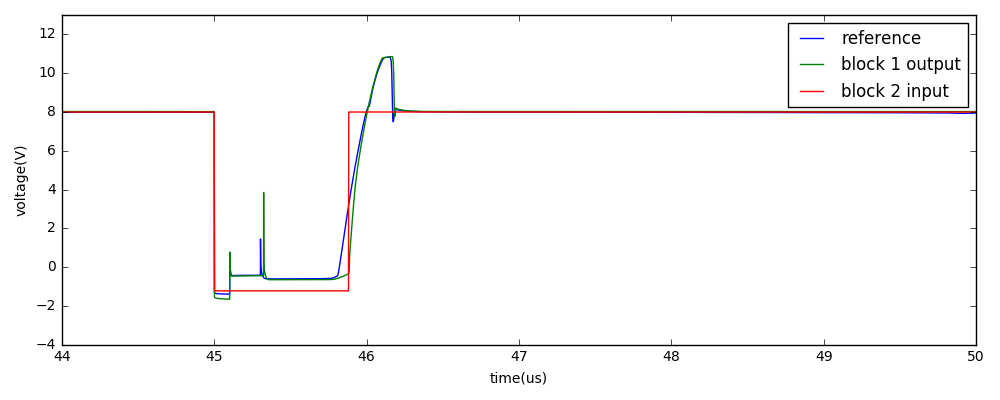
\includegraphics[width=0.98\textwidth]{src/1/figures/simulation_comparison_block1.png}
  \caption{Allure temporelle $V_{clamp9}$}
  \label{fig:sim-compare-block1}
\end{figure}

% Second block output
A la sortie du second bloc, des différences plus larges apparaissent entre la simulation individuelle (\textit{block 2 output}) et totale (\textit{reference}). (Fig. \ref{fig:sim-compare-block2}).
La courbe verte a une pente plus longue que la référence.
Néanmoins, les courbes ont quand même des caractéristiques communes en terme d'amplitude maximale et de durée, ce qui est intéressant en regard de cette méthode de modélisation.
La courbe de sortie est analysée et son amplitude maximale déterminée à 0 V avec une durée de 2 \textmugreek{}s.
Le stimulus appliqué sur le troisième bloc (le régulateur 2.5V) est également donné et porte le label \textit{block 3 input}).

\begin{figure}[!h]
  \centering
  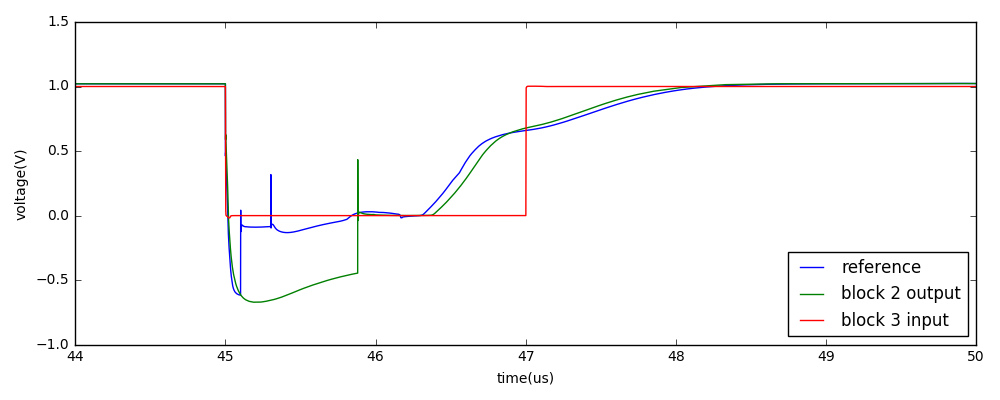
\includegraphics[width=0.98\textwidth]{src/1/figures/simulation_comparison_block2.png}
  \caption{Allure temporelle $V_{1p0}$}
  \label{fig:sim-compare-block2}
\end{figure}

La courbe de sortie du dernier bloc est donnée dans le document final, mais les résultats sont bons et les deux formes d'onde sont similaires, à un retard près.
Pour ce cas d'étude, il semblerait que la méthode de simulation et de modélisation individuelle permettrait par chainage des modèles d'estimer correctement la perturbation sur le bloc de sortie.
Avant de pouvoir généraliser son utilisation, il est nécessaire de tester cette méthode sur une plus large gamme d'applications.
Elle montre néanmoins des résultats prometteurs et pourrait faire l'objet d'études supplémentaires.

\section{Méthode boite noire}

Dans cette deuxième partie, la méthode boite-noire est présentée.
Elle a pour but de modéliser une fonction d'un circuit intégré, entre une entrée et une sortie.
L'objectif est d'effectuer une simulation ESD au niveau carte électronique, pendant le fonctionnement normal, en prenant en compte les circuits intégré.
Cette méthode nécessite de caractériser la fonction de transfert d'une fonction intégrée sur silicium, entre une broche d'entrée et une broche de sortie toutes deux externes.
Le principal avantage de cette méthode est de faire abstraction au niveau système de la complexité du circuit intégré.

% introduction, failure relation between input and output
La caractérisation est effectuée à nouveau avec une méthode Wunsch-Bell \cite{wunsch-bell} en appliquant une impulsion rectangulaire d'amplitude et de durée variables.
La broche d'entrée reçoit ce stress, pendant que la broche de sortie est surveillée et mesurée.
Contrairement à la méthode précédente, ici un critère de défaillance fixe est définie sur la sortie.
Dans cette étude, il consiste en un niveau de tension défini par la spécification de la fonction sous test.

% What is characterized
Pour tester cette méthode, elle est appliquée en simulation sur la schématique du véhicule de test détaillé dans le chapitre 3.
Les impulsions de caractérisation sont injectées sur l'entrée $V_{batt}$.
La broche de sortie à surveiller est la pin $V_{2p5}$, correspondant à l'alimentation 2.5 V régulée.
Le critère de défaillance est défini avec un seuil à 2.1 V en dessous duquel une faute est considérée.
En dessous de cette valeur sur $V_{2p5}$, les portes logiques alimentées par $V_{2p5}$ ne sont plus garanties de fonctionner correctement.
La figure \ref{fig:cz-black-box} affiche la présence d'une faute en fonction des paramètres du stress d'entrée.
L'axe des abscisses correspond à la largeur d'impulsion, et celui des ordonnées à l'amplitude du stress.
En soi, cette courbe peut être utilisée dans une simulation comme modèle de faute du bloc.
Avec une largeur d'impulsion et une amplitude appliquée sur $V_{batt}$, la courbe permet d'estimer ou non la présence d'une faute sur la sortie.

\begin{figure}[!h]
  \centering
  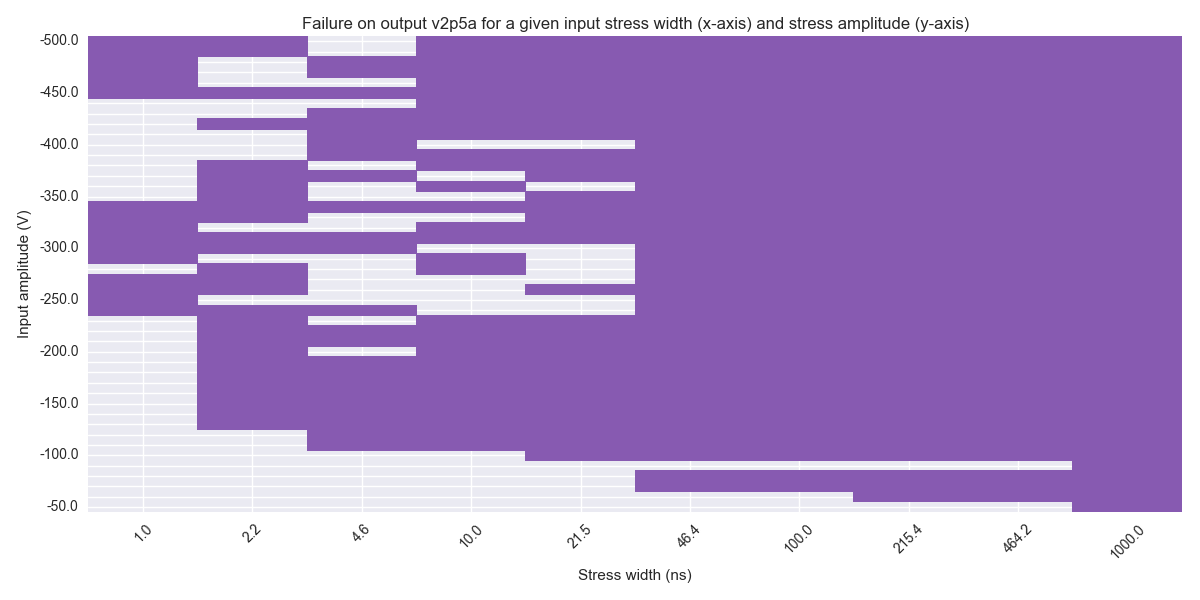
\includegraphics[width=\textwidth]{src/1/figures/black_box_regulator.png}
  \caption{Caractérisation boite-noire de la fonction de régulation}
  \label{fig:cz-black-box}
\end{figure}

% What to do with that
Néanmoins, l'objectif final de la méthode boite noire est aussi de fournir un modèle électrique équivalent du circuit intégré.
Le modèle de faute n'est pas un modèle électrique, et ne permet pas de déterminer par exemple pour une tension donnée quel courant est absorbé par une broche.
Sans un modèle électrique, il est impossible pour une personne externe d'effectuer une simulation ESD alimentée car alors il n'y a pas de modèle du circuit.
Par conséquent, il est aussi nécessaire de développer un modèle électrique équivalent de la broche.
Un modèle I(V) est proposé, extrait à partir de caractérisations effectuées avec la méthode TLP en simulation.
Les caractérisations sont très généralement effectuées sur des circuits non-alimentés.
Or ici, l'objectif est de simuler des modèles de circuit intégré en alimenté.
Pour évaluer l'impact de l'alimentation sur la caractérisation TLP, elle est effectuée à la fois sur un circuit alimenté et non alimenté.
La caractérisations de l'entrée dans les deux conditions d'alimentation est fournie Fig. \ref{fig:tlp-input-cz}.
Celle de la sortie est donnée dans le document final.

\begin{figure}[!h]
  \centering
  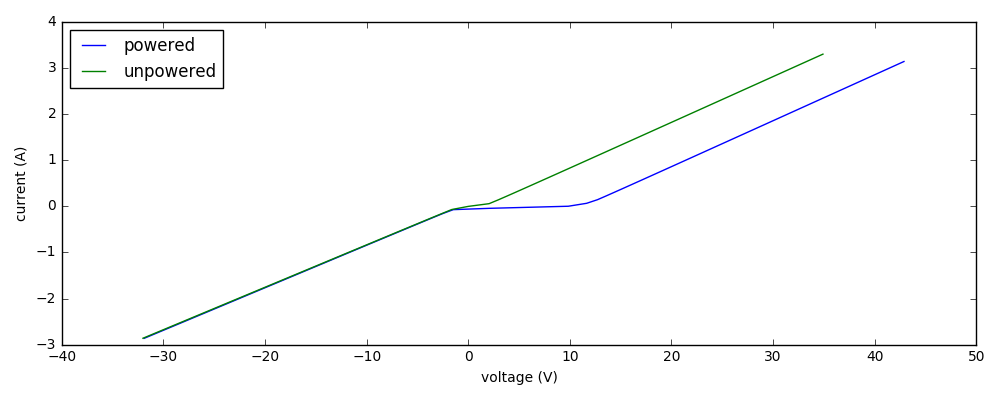
\includegraphics[width=\textwidth]{src/1/figures/tlp_input_characterization.png}
  \caption{caractérisation TLP de la broche d'entrée en alimenté et non-alimenté}
  \label{fig:tlp-input-cz}
\end{figure}

Pour l'entrée comme pour la sortie, des différences sont observées sur la courbe I(V) entre un circuit alimenté et non alimenté.
Des quantités différentes de courant sont absorbées par le circuit dans chaque condition.
Puisque le modèle est destiné à des simulations du composant en fonctionnement, la caractérisation en alimenté est sélectionnée par la suite.

% Explain the PWL model
Maintenant que le circuit est caractérisé, il est possible d'en construire un modèle électrique.
La stratégie utilisée est de reproduire la courbe I(V) avec une courbe linéaire par morceaux, en utilisant le langage de description matérielle Verilog-A.
Le code source du modèle est fourni dans le document complet.
% Validate the model with TLP
Le modèle est construit pour la broche d'entrée puis simulé et comparé à la schématique complète.
Il a été vérifié pour un amplitude de stress de 40 V (Fig. \ref{fig:compare-model-simu-m10}).
D'autres validations à -10 V et 40 V sont fournies dans le document complet.
Globalement, une bonne corrélation entre le modèle et le circuit complet est observée pour l'entrée.

\begin{figure}[!h]
  \centering
  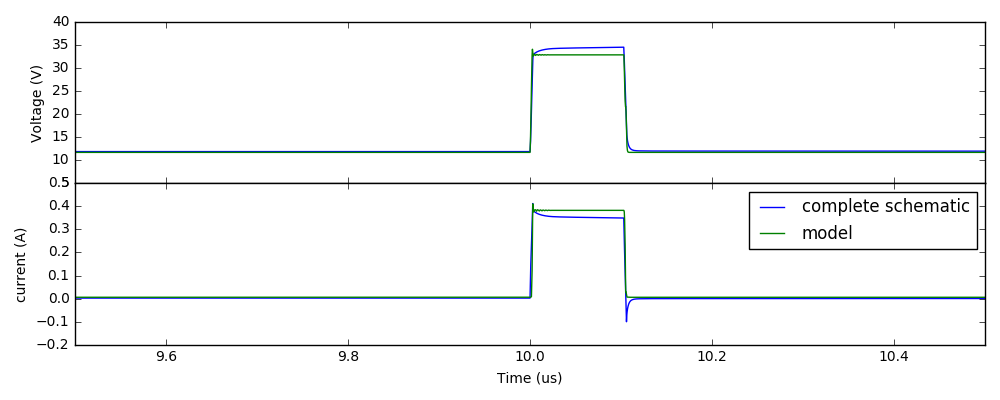
\includegraphics[width=\textwidth]{src/1/figures/comparison_model_total_40V.png}
  \caption{Comparaison entre la schématique complète et le modèle avec une injection TLP 40 V}
  \label{fig:compare-model-simu-m10}
\end{figure}

% Check the output
Contrairement à l'entrée, la sortie ne peut pas être modélisée par une simple courbe I(V) car elle est active et doit délivrer une tension à 2.5V.
Elle ne s'apparente pas à une impédance passive.
Pour reproduire ce comportement, un premier modèle est proposé Fig. \ref{fig:first-output-model}.
Il comporte une source de tension statique à 2.5V simulant la fonction de régulation.
La source de tension transitoire PWL n'est pas utilisée dans un premier temps, mais permet de simuler une faute et un redémarrage en venant modifier la tension de sortie.
Enfin, le modèle Verilog-A de courbe I(V) est connecté.
Une capacité de 100nF est connectée en sortie pour correspondre au schéma d'application classique de la fonction.

\begin{figure}[!h]
  \centering
  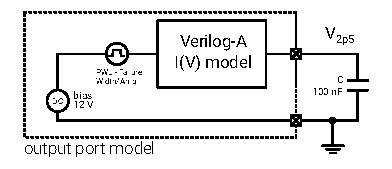
\includegraphics[width=0.7\textwidth]{src/1/figures/first_output_model.pdf}
  \caption{Modèle proposé pour la modélisation électrique de la sortie}
  \label{fig:first-output-model}
\end{figure}

% Is this first model working
Les tests montrent que ce modèle de la sortie ne fonctionne pas, car la combinaison de la courbe I(V) et de la source de tension 2.5V forcent un courant même si la tension de sortie est déjà à 2.5V.
Comme résultat la tension de sortie monte indéfiniment et la simulation n'est pas du tout précise.
Il est donc nécessaire de corriger la modélisation de la sortie et surtout l’interaction entre le modèle transitoire et le modèle DC.
Ce problèmes sera étudiés dans des travaux futurs afin d'être capable de proposer un modèle fonctionnel, pouvant servir pendant les phases de conception des cartes électroniques.

% Conclusion
Malgré les problèmes rencontrés durant les tests préliminaires, les modèles boite-noire restent une solution potentielle pour représenter le comportement d'une fonction intégré et pouvoir la distribuer sans révéler d'informations sensibles.
L'objectif s'intègre bien avec la méthodologie SEED (System Efficient ESD Design) \cite{seed} présentée en introduction, qui préconise de distribuer la responsabilité de la protection face aux ESD entre les circuits intégrés et les cartes électroniques.

Dans la première partie de ce chapitre, une méthode d'extraction de modèle de faute a été présentée.
Elle permet de créer des modèles boite-noire de la faute d'une fonction entre une entrée et une sortie.
Il y a énormément de possibilités d'expérimentation, et la méthode n'en est qu'à ses balbutiements, mais le concept de base semble efficace.
La seconde partie de la méthode consiste à modéliser et simplifier les entrées et sortie électriquement par d'une caractérisation TLP.
L'objectif est de réduire la complexité et les temps de simulation.
Cette méthode s'est avérée fonctionnelle pour la modélisation d'une entrée, mais ne fonctionne pas pour une sortie qui doit fournir du courant.
Des travaux et des investigations supplémentaires sont requises pour corriger ces problèmes.

% Opening work
Il y a énormément de pistes de recherche sur la modélisation boite-noire pour l'ESD.
Le comportement de ces modèles face à des impulsions plus variables tels que des décharges de pistolet ESD doit être étudié.
La méthode présentée doit être testée sur un plus grand nombre de fonctions analogiques, afin de voir si elle peut être appliquée généralement.
